% !TEX root = ./main.tex

\documentclass[12pt,a4paper]{report}

\usepackage[portuguese]{babel}
% \usepackage{hyphenat}
% \usepackage{amsmath}
\usepackage[compact]{titlesec}
% \usepackage[a4paper, margin=2.5cm]{geometry}
\usepackage{graphicx}

% \hyphenpenalty
% \exhyphenpenalty

\title{Trabalho Prático 1}

\newcommand{\subtitle}{Investigação Operacional} % Define subtitle (since it's not defined in the main file)

\date{\today}

\author{
    A104537 - Afonso Pedreira \\
    A104344 - Dário Guimarães \\
    A104365 - Fábio Magalhães \\
    A104534 - Hugo Rauber \\
    A104523 - Rodrigo Macedo
}

%% Define new command to show title, author and date
\makeatletter
\let\Title\@title
\let\Author\@author
\let\Date\@date
\makeatother

\newcommand{\makecover} {
    \begin{titlepage}
        \vspace*{0.5cm}

        %% Add your organization logo
        \raggedright % Align content to the left
        
\includegraphics[width=0.2\textwidth]{assets/images/uminho.png} % Adjust width as needed
        \hfill % Fill the space between image and text
        \parbox[b]{0.4\textwidth}{
            \raggedleft % Align content to the right
            \textbf{Universidade do Minho}\\
            Escola de Engenharia\\
            Departamento de Informática\\
            4710-057 Braga, Portugal
        }
        \vspace{2cm}
        
        %% Add your title, name, date, and organization
        \centering
        {\huge\bfseries \Title \par}
        \vspace{1cm}
        {\Large \subtitle \par}
        \vspace{1cm}
        {\large \Date \par}
        
        \vfill
        
        {\large \Author \par}
        
    \end{titlepage}
}


\begin{document}

% Para tirar "Capitulo X" antes de cada capitulo e diminuir espaço em cima:
\titleformat{\chapter}[display]   
{\normalfont\huge\bfseries}{\vspace{-50pt}}{20pt}{\Huge}
\titlespacing*{\chapter}{0pt}{0pt}{40pt}

\makecover

\tableofcontents

\newpage
    \chapter{Introdução}
    Este projeto está a ser desenvolvido no âmbito da unidade curricular de Investigação Operacional do ano 2023/2024, unidade esta que pretende dar a conhecer aos alunos os princípios fundamentais da otimização.

    \section{Motivação}
    A motivação para a realização deste projeto é a de aplicar os conhecimentos adquiridos ao longo do semestre, de forma a resolver um problema dado em contexto real.

\newpage
    \chapter{Desenvolvimento} 

    \section{Resolução do problema}
    \subsubsection{Modelo de Programação Linear}

    \subsection{Questão 0}
    Indique o valor de xABCDE, e apresente duas tabelas como as do enunciado com os valores
    resultantes da aplicação da regra. Calcule também a soma dos comprimentos dos itens a empacotar.
    \subsubsection*{Resposta:}
    \subsubsection*{Regra para determinar as listas de contentores e de itens:}
    Seja xABCDE o número de inscrição do estudante do grupo com maior número de inscrição, (\textbf{no caso atual, o número 104537; resultante em x = 1; A = 0; B = 4; C = 5; D = 3; E = 7}). O número de contentores disponíveis de cada comprimento e o número de itens
    a empacotar de cada comprimento são dados pelas seguintes tabelas:

    \begin{table}[h]
        \centering
        contentores \\
        \begin{tabular}{|c|c|}
        \hline
        \textbf{comprimento} & \textbf{quantidade disponível} \\
        \hline
        11 & ilimitada \\
        10 & 5 (B+1) \\
        7 & 4 (D+1) \\
        \hline
        \end{tabular}
    \end{table}

    \begin{table}[h]
        \centering
        itens \\
        \begin{tabular}{|c|c|}
        \hline
        \textbf{comprimento} & \textbf{quantidade} \\
        \hline
        1 & $k_1$=0 (se o algarismo B for par, então k1 = 0, senão k1 = 2;) \\
        2 & $k_2$=13 (se o algarismo C for par, então k2 = C+2, senão k2 = C+8;) \\
        3 & $k_3$=10 (se o algarismo D for par, então k3 = 0, senão k3 = 10;) \\
        4 & $k_4$=15 (se o algarismo E for par, então k4 = E+2, senão k4 = E+8;) \\
        5 & 5 \\
        \hline
        \end{tabular}
    \end{table}

    Soma dos comprimentos dos itens a empacotar: $k_1 + k_2 + k_3 + k_4 + 5 = 0 + 13 + 10 + 15 + 5 = 43$

    \subsection{Questão 1}
    Apresente a formulação deste problema.
    \subsubsection*{Resposta:}
    Neste problema, pretende-se minimizar a quantidade de contentores utilizados para empacotar um conjunto de itens, de forma a minimizar o desperdício de espaço.
    Para tal, é necessário determinar a quantidade de contentores de cada comprimento a utilizar, bem como a quantidade de itens a empacotar de cada comprimento.
    O problema pode ser formulado como um problema de programação linear, com o objetivo de minimizar a função objetivo:
    \begin{equation}
        \text{min} \sum_{i=1}^{n} k_i x_i
    \end{equation}

    onde $k_i$ é comprimento do item i, e $x_i$ é o número de contentores de comprimento $k_i$ a utilizar.

    Sujeito às seguintes restrições:

    \begin{equation}
        \sum_{i=1}^{n} x_i \geq \sum_{i=1}^{n} k_i
    \end{equation}

    \subsection{Questão 2}
    Apresente o modelo de programação linear.
    \subsubsection*{Resposta:}
    <resposta text here>

    \subsection{Questão 3}
    Apresente o ficheiro de input (cut-and-paste).
    \subsubsection*{Resposta:}
    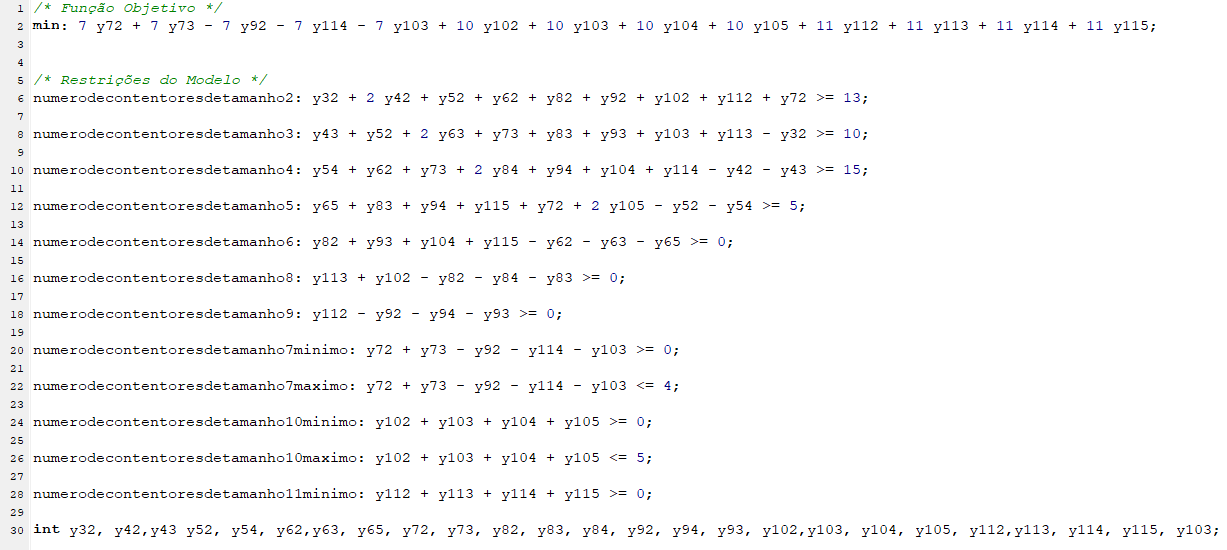
\includegraphics[width=1.2\textwidth]{assets/images/lp_code.png}

    \subsection{Questão 4}
    Apresente o ficheiro de output produzido pelo programa (cut-and-paste).
    \subsubsection*{Resposta:}
    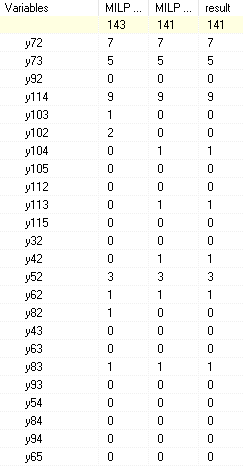
\includegraphics[width=0.4\textwidth]{assets/images/lp_sol.png}

    \subsection{Questão 5}
    Interprete a solução óptima, indique a soma dos comprimentos dos contentores usados, e
    apresente um plano do empacotamento em que cada contentor utilizado é representado por
    uma barra com o comprimento do contentor, mostrando a forma como é dividido para obter
    o conjunto de itens nele colocados.
    \subsubsection*{Resposta:}
    <resposta text here>

    \subsection{Questão 6}
    Descreva os procedimentos usados para validar o modelo
    \subsubsection*{Resposta:}
    <resposta text here>

\newpage
    \chapter{Conclusão}
        <conclusão text here>

\end{document}